\documentclass[12pt,a4paper,openright]{report}
\usepackage[italian]{babel}
\usepackage{newlfont}
\usepackage[utf8]{inputenc}
\usepackage{fancyhdr}
\usepackage{indentfirst}
\usepackage{showkeys}
\usepackage{amssymb}
\usepackage{amsmath}
\usepackage{latexsym}
\usepackage{amsthm}
\usepackage{qcircuit}
\usepackage{braket}
\usepackage{kbordermatrix}
\usepackage{relsize}
\usepackage{listings}
\usepackage{color}
\usepackage{graphicx}
\usepackage{tikz}
\usepackage{caption}
\captionsetup[figure]{labelformat=empty}
\usetikzlibrary{arrows,shapes.gates.logic.US,shapes.gates.logic.IEC,calc}
\definecolor{dkgreen}{rgb}{0,0.6,0}
\definecolor{gray}{rgb}{0.5,0.5,0.5}
\definecolor{mauve}{rgb}{0.58,0,0.82}
\renewcommand{\chaptermark}[1]{\markboth{\thechapter.\ #1}{}}
\renewcommand{\sectionmark}[1]{\markright{\thesection \ #1}{}}
\newcommand*{\field}[1]{\mathbb{#1}}
\newcommand*\xor{\mathbin{\oplus}}
\newcommand*\Mycomb[2]{\prescript{#1\mkern-0.5mu}{}C_{#2}}
\newtheorem{mydef}{Definizione}[chapter]
\newtheorem{mylem}{Lemma}
\newtheorem*{mycor}{Corollario}
\newtheorem{mythm}{Teorema}
\pagestyle{fancy}\addtolength{\headwidth}{30pt}
\rhead[\fancyplain{}{\bfseries\leftmark}]{\fancyplain{}{\bfseries\thepage}}
\cfoot{}
%%%%%%%%%%%%%%%%%%%%%%%%%%%%%%%%%%%%%%%%%
\linespread{1.3}                        %comando per impostare l'interlinea
%%%%%%%%%%%%%%%%%%%%%%%%%%%%%%%%%%%%%%%%%definisce nuovi comandi
%
\textwidth=450pt\oddsidemargin=0pt
\begin{document}
\begin{titlepage}
\begin{center}
{{\Large{\textsc{Alma Mater Studiorum $\cdot$ Universit\`a di
Bologna}}}} \rule[0.1cm]{15.8cm}{0.1mm}
\rule[0.5cm]{15.8cm}{0.6mm}
{\small{\bf SCUOLA DI SCIENZE\\
Corso di Laurea in Informatica }}
\end{center}
\vspace{15mm}
\begin{center}
{\LARGE{\bf TITOLO}}\\
\vspace{3mm}
{\LARGE{\bf DELLA}}\\
\vspace{3mm}
{\LARGE{\bf TESI}}\\
\end{center}
\vspace{40mm}
\par
\noindent
\begin{minipage}[t]{0.47\textwidth}
{\large{\bf Relatore:\\
Chiar.mo Prof.\\
UGO DAL LAGO}}
\end{minipage}
\hfill
\begin{minipage}[t]{0.47\textwidth}\raggedleft
{\large{\bf Presentata da:\\
FEDERICO PECONI}}
\end{minipage}
\vspace{20mm}
\begin{center}
{\large{\bf II Sessione\\%inserire il numero della sessione in cui ci si laurea
a.a. 2016/2017 }}%inserire l'anno accademico a cui si è iscritti
\end{center}
\newpage
\thispagestyle{empty}                   %elimina il numero della pagina
\topmargin=6.5cm                        %imposta il margina superiore a 6.5cm
\raggedleft                             %incolonna la scrittura a destra
\large                                  %aumenta la grandezza del carattere
                                        %   a 14pt
\em                                     %emfatizza (corsivo) il carattere
Questa \`e la \textsc{Dedica}:\\
ognuno pu\`o scrivere quello che vuole, \\
anche nulla \ldots                      %\ldots lascia tre puntini
\newpage                                %va in una pagina nuova
%
%%%%%%%%%%%%%%%%%%%%%%%%%%%%%%%%%%%%%%%%
\clearpage{\pagestyle{empty}\cleardoublepage}%non numera l'ultima pagina sinistra
\end{titlepage}
\tableofcontents
\chapter{Introduzione}
\chapter{Funzioni Booleane Bilanciate}
Come già anticipato nell'Introduzione, le funzioni Booleane bilanciate sono una struttura matematica su cui poggia parte del contenuto di questa tesi.
É risultato perciò utile, ai fini di una trattazione chiara ed esaustiva, impiegare un capitolo per definirne in maniera rigorosa i concetti di base.\\
"\textit{Per fare un tavolo ci vuole il legno}" recita l'inizio di una famosa canzone per bambini, ad indicare la natura celata delle cose che, così nella quotidianità
come nella matematica, spesso necessitano di altre conoscenze per essere comprese appieno; seguendo quindi questa impronta fondazionale, andiamo per prima cosa ad introdurre le funzioni Booleane.

\section{Funzioni Booleane}
Le funzioni Booleane apparvero per la prima volta a metà 19esimo secolo durante la formulazione matematica di problemi logici e prendono
il loro nome da George Boole, matematico britannico considerato fondatore della logica matematica odierna\cite{ref2}.\newpage
Una semplice funzione Booleana può può essere rappresentata da \\$f:\{0,1\}^2 \mapsto \{0,1\}$
\begin{align*}
    f(00) = 0 \\
    f(01) = 0 \\
    f(10) = 1 \\
    f(11) = 0
\end{align*}
oppure da $f^\prime:\{TRUE,FALSE\}\mapsto{\{TRUE,FALSE\}}$
\begin{align*}
    f^\prime(FALSE) = TRUE \\
    f^\prime(TRUE) = FALSE 
\end{align*}
Notiamo come entrambe abbiano in comune la dimensione del codominio e la capacità di agire su un numero finito di valori appartenenti ad un insieme di 2 elementi.
È tuttavia conveniente operare su di un insieme che possa essere visto sia dal punto di vista qualitativo (vero, falso)
sia da un punto di vista quantitativo, e quindi numerico, che ci permetta così di compiere anche operazioni algebriche oltre che logiche. Prediligeremo allora da qui in avanti l'inisieme
$\{0,1\}$ come campo vettoriale su cui lavorare.
\par
\begin{mydef}
    Una \textnormal{funzione Booleana a \textit{n} variabili} è una funzione da $\mathcal{B}^n$ a $\mathcal{B}$,
    dove $\mathcal{B} = \{0,1\}$, $n > 0$ e $\mathcal{B}^n$ è l'n-esimo prodotto cartesiano di $\mathcal{B}$ con se stesso.\cite{ref3}
\end{mydef}
\begin{mycor}
    $\forall$ $n > 0$, ci sono $2^{2^{n}}$ funzioni da $\mathcal{B}^n$ a $\mathcal{B}.$
\end{mycor}
\begin{proof}
    Sia $\mathcal{F}=\{f|f:\mathcal{B}^n\mapsto{\mathcal{B}}\}$,
    ogni $f$ riceve in input n-uple $\vec{x}=(x_1,..,x_n)$ che possono essere viste come sequenze di $n$ bit.
    In $n$ bit possiamo codificare, trattandosi di una distribuzione con ripetizione di classe $n$, $2^n$ oggetti differenti, quindi $\mathbb{D}_{2,n}=\left\vert{\mathcal{B}^n}\right\vert = 2^n$.
    Per definizione di $f$, per ogni $\vec{x}$, $f(\vec{x}) = 0$  oppure  $f(\vec{x}) = 1$, quindi ogni possibile $f$ individua un sottoinsieme di $\mathcal{B}^n$.\\
    Allora $\mathcal{F}$ avrà caridinalità uguale all'insieme delle parti per $\mathcal{B}^n$, quindi  $\left\vert{\mathcal{F}}\right\vert = 2^{\mathcal{B}^n}=2^{2^{n}}$

\end{proof}
Un altro modo più tradizionale per descrivere una funzione Booleana è quello di fornire la sua tabella di verità.
Ad esempio, per la $f$ precedentemente definita, la tabella di verità relativa sarà:


\begin{displaymath}
    \begin{array}{|c|c|c|}\hline
        x_1 & x_2 & f(x_1, x_2) \\\hline 
        0   & 0   &  0  \\ 
        0   & 1   &  0  \\
        1   & 0   &  1  \\
        1   & 1   &  0  \\\hline
    \end{array}
\end{displaymath}
Dove a destra viene posto il risultato della funzione calcolata sui valori delle colonne precedenti.\par
In entrambe le rappresentazioni, tuttavia, le funzioni vengono descritte in maniera implicita mostrando solamente input ed output,
senza mai andare a specificare come questo output venga calcolato.\\
Nell'ultimo capitolo, per l'implementazione dell'algoritmo di Deutsch-Jozsa, verranno utilizzate funzioni Booleane \textit{bilanciate}
che necessitano di essere calcolate esplicitamente. La prossima sezione introduce questa categoria di funzioni Booleane e 
propone due metodi effettivi e generali per produrne istanze concrete.

\section{Classi di Funzioni Booleane Bilanciate}

Sia $f$ una funzione Booleana, chiamiamo $\vec{x}=(x_1,..,x_n)$ \textit{vettore positivo} per $f$ se e solo se
$f(\vec{x}) = 1$, \textit{vettore negativo} altrimenti. Sia $({\left\vert{f}\right\vert}^1 \text{,} {\left\vert{f}\right\vert}^0)$ la partizione dove ${\left\vert{f}\right\vert}^1$ è la quantità che indica il numero di vettori
positivi per $f$ e ${\left\vert{f}\right\vert}^0$ la quantità che indica il numero di vettori negativi.
\begin{mydef}
    Una funzione Booleana $f$ è detta bilanciata (FBB) se e solo se ${\left\vert{f}\right\vert}^1 = {\left\vert{f}\right\vert}^0$.
\end{mydef}
\begin{mycor}
    $\forall$ $n > 0$, ci sono $\frac{2^{n}!}{(2^{n-1}!)^2}$ FBB da $\mathcal{B}^n$ a $\mathcal{B}.$
\end{mycor}
\begin{proof}
    Per definizione, una FBB $fbb:\mathcal{B}^n\mapsto\mathcal{B}$ è individuata da una partizione $(\mathcal{M},\mathcal{N})$ con $\mathcal{M}\subset\mathcal{B}^n$ e $\mathcal{N}\subset\mathcal{B}^n$ tale che
    $\left\vert{\mathcal{M}}\right\vert = \left\vert{\mathcal{N}}\right\vert = 2^{n-1}$ e $fbb(m)=0 \land fbb(n)=1$ $\forall{m,n}$ con $m\in\mathcal{M},n\in\mathcal{N}$.
    Quindi, il numero delle possibili funzioni corrisponde a tutti i possibili modi di partizionare a metà un insieme di $2^n$ elementi e, a sua volta, ogni partizione così creata può essere rappresentata 
    da un sottoinsieme $\mathcal{S}\subset\mathcal{B}^n$ dove $\mathcal{M}=\mathcal{S}$ e $\mathcal{N}=\mathcal{B}^n \setminus \mathcal{S}$.
    Non resta quindi che trovare tutti i possibili $\mathcal{S}$:  
    \begin{center}
    \[
        \mathbb{C}_{2^n,2^{n-1}}= \binom{2^n}{2^{n-1}} = \frac{2^n!}{2^{n-1}!2^{n-1}!} = \frac{2^n!}{(2^{n-1}!)^2}
    \]
    \end{center}
\end{proof}
Una valida tabella di verità per una FBB in $\mathcal{B}^3$ portebbe essere la seguente:

\begin{center}
\scalebox{0.90}{$
    \begin{array}{|c|c|}\hline
        (x_1,x_2,x_3) & g(x_1,x_2,x_3) \\\hline 
        (0,0,0)         &  0  \\ 
        (0,0,1)         &  1  \\
        (0,1,0)         &  1  \\
        (0,1,1)         &  0  \\    
        (1,0,0)         &  1  \\
        (1,0,1)         &  0  \\
        (1,1,0)         &  0  \\
        (1,1,1)         &  1  \\\hline
    \end{array}$
}
\end{center}
Dove, giustamente, si noti come il numero dei vettori positivi equivale al numero dei vettori negativi.\par
Ma come è costruita $g$ nello specifico? Qual'è la computazione che mi porta a determinati outputs?
Per rispondere a queste domande si può provare a cercare qualche correlazione tra i valori in entrata e i valori in uscita:
dopo un pò di riflessione dovrebbe saltare all'occhio che ogni qual volta abbiamo un numero dispari di $1$ nell'input la funzione 
restituisce $1$, restituisce invece $0$ quando tale numero è pari.
La parità di una sequenza è esprimibile con la somma modulo $2$ dei singoli componenti, allora possiamo definire esplicitamente $g$ come:
\begin{align*}
    g(x_1, x_2, x_3)= &x_1 + x_2 + x_3 \mod 2  \\
                    = &(x_1 \xor x_2) \xor x_3  \\
                    = &x_1 \xor x_2 \xor x_3
\end{align*}
dove $\xor$ è un connettivo binario logico (una funzione Booleana $\in \mathcal{B}^2$) chiamato XOR oppure OR esclusivo, che restituisce $1$ se uno ed uno solo dei due 
elementi vale $1$. 

\begin{center}
    \scalebox{0.90}{$
        \begin{array}{|c|c|}\hline
            (x_1,x_2) & \xor(x_1,x_2) \\\hline 
            (0,0)         &  0  \\ 
            (0,1)         &  1  \\
            (1,0)         &  1  \\
            (1,1)         &  0  \\\hline    
        \end{array}$
    }
    \end{center}
\par
\begin{mylem}
    Per ogni $n > 0$ la funzione Booleana $ f^{n}(x_1,x_2,...,x_n) = x_1 \xor x_2 \xor ... \xor x_n $ è una FBB.  
\end{mylem}
\begin{proof}
    \textit{(per induzione su $n$)\\}
    \begin{description}
        \item[Base induttiva:] $f^1(x)=x$ è trivialmente bilanciata.
        \item[Ipotesi induttiva:] Ipotizziamo $f^n$ bilanciata, quindi esiste la partizione $(\mathcal{M},\mathcal{N})$ con $\mathcal{M}\subset\mathcal{B}^n$ e $\mathcal{N}\subset\mathcal{B}^n$ tale che:\\
                                      ${\left\vert{\mathcal{M}}\right\vert} = {\left\vert{\mathcal{N}}\right\vert}$, $\mathcal{M} \cup \mathcal{N} = \mathcal{B}^n$ e $\forall m,n$ con
                                      $m\in\mathcal{M}$,$n \in\mathcal{N}$ risulta $f^n(m) = 0$ e $ f^n(n) = 1$.
        \item[Passo induttivo:] Avremo $f^{n+1}:\mathcal{B}^{n+1}\mapsto\mathcal{B}$ dove  $\mathcal{B}^{n+1} = \mathcal{B}^n\cdot0 \cup \mathcal{B}^n\cdot1$ e quindi\\
                                     $\left\vert\mathcal{B}^{n+1}\right\vert = 2\left\vert\mathcal{B}^{n}\right\vert$. Dobbiamo dimostrare che esiste una partizione
                                     $(\mathcal{M^\prime},\mathcal{N^\prime})$ t.c.:
                                     \begin{itemize}
                                        \item $\left\vert\mathcal{M^\prime}\right\vert=\left\vert\mathcal{B}^{n}\right\vert$ e $\forall m^\prime \in \mathcal{M^\prime}$ $f^{n+1}(m^\prime) = 0$ 
                                        \item $\left\vert\mathcal{N^\prime}\right\vert=\left\vert\mathcal{B}^{n}\right\vert$ e $\forall n^\prime \in \mathcal{N^\prime}$ $f^{n+1}(n^\prime) = 1$   
                                      \end{itemize}
                                      Notiamo come, $\forall m,n$ con $ m\in\mathcal{M},n\in\mathcal{N}$ se\\
                                      $x_{n+1} = 0 \Rightarrow $ $f^{n+1}(m\cdot0)=0 \land f^{n+1}(n\cdot0)=1$\\
                                      $x_{n+1} = 1 \Rightarrow $$f^{n+1}(m\cdot1)=1 \land f^{n+1}(n\cdot1)=0$\\
                                      Segue naturalmente che la partizione $\mathcal{M^\prime} = \mathcal{M}\cdot0 \cup \mathcal{N}\cdot1$ e $\mathcal{N^\prime} = \mathcal{M}\cdot1 \cup \mathcal{N}\cdot0$
                                      rispetta i criteri cercati. 
    \end{description}      
\end{proof}
\par
Si richiami dall'Algebra Lineare che, $f:\mathcal{V}\mapsto\mathcal{W}$ è un'applicazione lineare se e solo se esiste una matrice $M \in \mathbb{M}^{k \times l}$ tale che $f(\vec{x})=M\vec{x}$, dove $k = \left\vert\mathcal{V}\right\vert$ e $l = \left\vert\mathcal{W}\right\vert$ sono le dimensioni degli spazi vettoriali su cui agisce.\\

\begin{mydef}
$b:\mathcal{B}^n \mapsto \mathcal{B}$ è una funzione booleana lineare (FBL) se e solo se esiste $M \in \mathbb{B}^{n \times 1}$ tale che $b(\vec{x})=M\vec{x}=c_1x_1+c_2x_2+,...,+c_nx_n=(c_1\land{x_1})\xor(c_2\land{x_2})\xor,...,\xor(c_n\land{x_n})$. Dove $\xor$
è l'operatore di somma per $\mathcal{B}^n$. 
\end{mydef}
\begin{mycor}
    Per ogni $n>0$, $f^n$ è una FBL.
    \begin{proof}
        Triviale, basta infatti porre $M=\overbrace{(1,1,...,1)}^{n-volte}$.
    \end{proof}
\end{mycor}

\subsection{La Classe delle Funzioni Booleane Lineari}
Introdotte le FBB e le FLB, possiamo a questo punto procedere con la formulazione del seguente risultato generale:
\begin{mythm}
    Sia $\mathbb{FL}=\{f|f\in\text{FLB} \land f \neq c:\mathcal{B}^n\mapsto\{0\},\;\forall n > 0\}$ la classe di tutte le funzioni Booleane lineari
    diverse dalle funzioni costanti a 0. Allora, $\forall f\in \mathbb{FL}$ $f$ è bilanciata.
\end{mythm}
\begin{proof} \textit{(per induzione su $n$)\\}
    Sia $l^n$ una qualsiasi funzione da $\mathcal{B}^n$ appartenente a $\mathbb{FL}$.  Vogliamo dimostrare che $l^n$ è sempre bilanciata.\\
    \begin{description}
        \item[Base induttiva:] $l^1(x)=x$ è trivialmente bilanciata.
        \item[Ipotesi induttiva:] Ipotizziamo $l^n$ bilanciata.\\
                                      Esisterà quindi la partizione $(\mathcal{M},\mathcal{N})$ con $\mathcal{M}\subset\mathcal{B}^n$ e $\mathcal{N}\subset\mathcal{B}^n$ tale che:\\
                                      ${\left\vert{\mathcal{M}}\right\vert} = {\left\vert{\mathcal{N}}\right\vert}$, $\mathcal{M} \cup \mathcal{N} = \mathcal{B}^n$ e $\forall m,n$ con
                                      $m\in\mathcal{M}$,$n \in\mathcal{N}$ risulta $l^n(m) = 0$ e $ l^n(n) = 1$.
        \item[Passo induttivo:] Il passo chiave sta nel notare che $l^{n+1}$ può assumere esclusivamente una delle seguenti forme:
                                \begin{itemize}
                                    \item \textbf{Singoletto} $\Rightarrow$ $l^{n+1}(\vec{x}) = l^{n+1}(x_1,x2,...,x_{n+1})=x_{n+1}$\\
                                                              Che è bilanciata in quanto, sia $(\mathcal{M},\mathcal{N})$ la partizione dove $\mathcal{M}$ è composto da tutte le stringhe
                                                              binarie $\in \mathcal{B}^{n+1}$ che codificano in base due i numeri da $0$ a $2^n - 1$ e $\mathcal{N}$ composto da tutte le stringhe binarie
                                                              $\in \mathcal{B}^{n+1}$ che codificano in base due i numeri da $2^n$ a $2^{n+1} - 1$ i.e. :\\
                                                              $\mathcal{M}= \{\vec x \in \mathcal{B}^{n+1} | \vec x = 0\cdot x_n \cdot x_{n-1}\cdot ...\cdot x_1\}$\\
                                                              $\mathcal{N}= \{\vec x \in \mathcal{B}^{n+1} | \vec x = 1\cdot x_n \cdot x_{n-1}\cdot ...\cdot x_1\}$\\
                                                              Allora $\mathcal{M}\subset\mathcal{B}^{n+1}$ e $\mathcal{N}\subset\mathcal{B}^{n+1}$, ${\left\vert{\mathcal{M}}\right\vert} = {\left\vert{\mathcal{N}}\right\vert}$, $\mathcal{M} \cup \mathcal{N} = \mathcal{B}^{n+1}$ e
                                                              e $\forall m,n$. $m\in\mathcal{M}$,$n \in\mathcal{N}$ risulta $l^{n+1}(m) = 0$ e $ l^{n+1}(n) = 1$.
                                    \item \textbf{Uguale a $l^n$} $\Rightarrow$ Bilanciata per ipotesi. 
                                    \item \textbf{Xor di $l^n$} $\Rightarrow$ $l^{n+1}(\vec{x}) = l^{n+1}(x_1,x2,...,x_{n+1})= x_{n+1} \xor l^n$.
                                    \\ E quindi se:\\
                                    $x_{n+1} = 0 \Rightarrow l^{n+1} = 0 \xor l^n = l^n$ \\
                                    $x_{n+1} = 1 \Rightarrow l^{n+1} = 1 \xor l^n = \neg l^n$\\
                                    Individuiamo, concludendo la dimostrazione, la partizione cercata $(\mathcal{M^\prime},\mathcal{N^\prime})$ con:\\
                                    $\mathcal{M^\prime} = M\cdot0 \cup N\cdot1 \:\:$  e  $\:\: \mathcal{N^\prime} = M\cdot1 \cup N\cdot0$.
                                \end{itemize}
    \end{description}
\end{proof}
\noindent Questo significa che, qualsiasi siano i coefficienti della nostra FBL, a patto che questi non siano tutti $0$, produrrano una funzione bilanciata.\par

Giunti a questo punto è lecito domandarsi se esistano altre (semanticamente diverse) FBB  non lineari e se sì, quante ne si possono ancora trovare?
Il numero di FBL per $n$ fissato, equivale al numero di \textit{disposizioni con ripetizione di classe} $n$ (coefficienti) da un insieme di due elementi $\{0,1\}$ meno la disposizione $M^*=\overbrace{(0,0,...,0)}^{n-volte}$ che identifica la costante 0, cioè $\mathbb{D}_{2,n}-1= 2^n - 1$.
Tale numero è chiaramente inferiore al numero di FBB : $\mathbb{C}_{2^n,2^{n-1}}$ ricavato dal Corollario 2.2. E quindi sì, esisteranno sicuramente, per ogni $n$, $\mathbb{C}_{2^n,2^{n-1}} - (\mathbb{D}_{2,n} - 1)$ FBB non lineari.

\subsection{Funzioni Booleane non Lineari Bilanciate}
L'approfondimento delle proprietà e della teoria riguardante il vasto campo di studi delle funzioni Booleane, per quanto interessante, esula dai fini della tesi in oggetto.
Rimanendo in tema, tuttavia, è bene accennare che la ricerca, specie per quanto riguarda l'indagine sulle funzioni booleane bilanciate è molto attiva e di fondamentale importanza in applicazioni come la crittografia a chiave simmetrica.\cite{ref4}.\\
Per rendere più realistica e articolata l'implementazione degli script presentati nel Capitolo 5, si è optato per la ricerca in letteratura di funzioni booleane bilanciate non lineari
da utilizzare nell'algoritmo di Deutsch-Jozsa. In particolare, è stata scelta una funzione a 5 variabili, ricavata con il metodo generale esposto da \textit{Logachev}\cite{ref5}:
    \begin{align*}
            h(x_1, x_2, x_3, x_4, x_5)=(x_1 \land x_2) \xor x_3 \xor (x_2 \land x_3 \land x_4) \xor (x_2 \land x_3 \land x_5) \xor (x_3 \land x_4) \xor (x_4 \land x_5)
    \end{align*}



\begin{figure}[h]
     \centering
     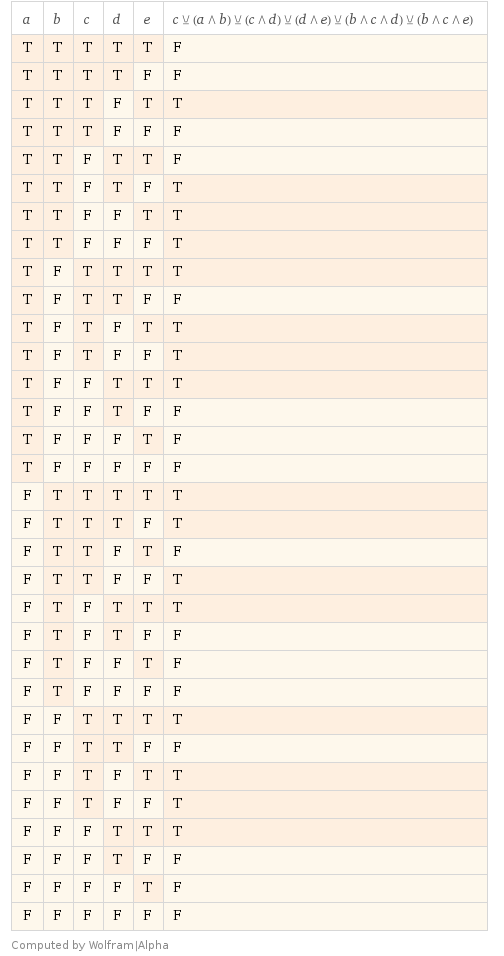
\includegraphics[width=0.5\textwidth,height=13.1cm]{computedFBBtrueTable}
     \caption{Tabella di verità per $h$}
\end{figure}
    

\chapter{L'Informazione Quantistica}
Questa tesi si sviluppa nel contesto dell'Informazione Quantistica.\\
L'Informazione Quantistica è una nuova branca di studi della teoria dell'informazione che trova la sua collazione nell'intersezione tra
Fisica, Matematica e Informatica.\\
La nascita di questo nuovo campo di studi è dovuta in gran parte alle intuizioni del celeberrimo fisico Richard Feynmann, il quale fu il primo a suggerire,
in una sua lezione nel 1981 \cite{ref6}, che il tipo di computer ideale che fosse stato capace di simulare i fenomeni naturali in maniera
efficiente sarebbe stato un computer che avesse risposto alle stesse leggi della meccanica quantistica. L'argomento da lui proposto faceva
perno sulla natura esponenziale che il mondo subatomico presenta se osservato dal punto di vista macroscopico e che quindi, avrebbe portato,
per un processo transitivo, qualsiasi computer classico a sperimentare un tempo altrettanto esponenziale per simularlo.\\
Spinti da questa osservazione, numerosi ricercatori si cimentarono nello studio e nella formalizzazione di questo nuovo paradigma di calcolo,
gettandone le basi teoriche: nel 1982, Paul Benioff, nell'articolo "Quantum mechanical models of Turing machines that dissipate no energy"\cite{ref7}, 
dimostrò come un sistema basato sulla meccanica quantistica avrebbe potuto modellare una macchina di Turing (MdT) senza dissipare energia (il concetto della conservazione dell'energia 
verrà ripreso e chiarito in seguito). In altre parole, questi dimostrò come la meccanica quantistica fosse sufficiente ad esprimere il più
famoso dei modelli tradizionali di calcolo, ma poteva fare addirittura di meglio? \\
All'incirca nello stesso momento il fisico David Deutsch rispose a tale quesito introducendo prima la controparte quantica della MdT universale (QMdTU)
e poi dimostrando che la QMdTU riusciva a compiere operazioni al di fuori della portata della MdTU, come generare in maniera genuina numeri random,
performare calcoli paralleli su di un unico registro e simulare perfettamente sistemi fisici a stati di dimensione finita, confermando così
la visionaria congettura che Feynmann aveva sollevato solo pochi anni prima.  

\section{Principi della Meccanica Quantistica}
Nel mondo microscopico, quando si scende sotto la soglia atomica, cominciano ad emergere fenomeni che sono difficilmente interpretabili utilizzando il solo senso comune,
le nozioni più elementari come la determinazione unica delle proprietà fisiche di un oggetto (velocità, posizione, ecc.) a cui siamo abituati fin da piccoli non sono più le stesse e
postulati come il principio di località o il determinismo, cessano di essere veri.
Ciò portò inizialmente esponenti eminenti del campo (del calibro di Einstein) a guardare con scetticismo o addirittura a rifiutare la meccanica quantistica per via delle stranezze a cui essa portava.
Numerosi esperimenti condotti successivamente hanno tuttavia confermato con successo più volte le previsioni della teoria e ad oggi, nella comunità scientifica vi è unanime consenso sulla veriditicità di questa.\\
Al fine di capire il calcolo quantistico è necessario per prima cosa acquisire familiarità con queste nuove leggi fondamentali che governano il mondo dei quanti.
Vengono di seguito esposte sinteticamente le caratteristiche peculiari della meccanica quantistica e, di seguito in maniera più formale, il modo in cui queste influenzano l'Informatica.

\subsection{Dai Numeri Reali ai Numeri Complessi}
La meccanica quantistica differisce dalla maggior parte delle branche della scienza per via del largo uso che fa dei numeri complessi.
I numeri complessi vennero per la prima volta introdotti come una curiosità matematica: $i=\sqrt{-1}$, chiamata unità immaginaria, era la soluzione "immaginaria" postulata
all'equazione $x^2=-1$. Per tanto tempo il campo dei numeri complessi è rimasto confinato unicamente nel reame della matematica fino a quando,
con lo studio sistematico delle funzioni d'onda e l'introduzione delle analisi di Fourier, ci si accorse che i numeri complessi erano la struttura
ottimale per descrivere in maniera compatta un'onda. Inizialmente la meccanica quantistica fece largo uso delle funzioni d'onda.\par
\begin{mydef}
    Un numero complesso $\text{c}$ è un'espressione
    \begin{center}
        $c = a + b \times i = a + bi$\\
    \end{center}
        dove $a$ e $b$ sono due numeri reali, $a$ è chiamata la parte reale di $c$, mentre $b$ è la parte immaginaria.
    
\end{mydef}
Uno stato quantico è rappresentato da vettori unitari in uno spazio vettoriale complesso.

\subsection{Da Stati Singoli alla Sovrapposizione degli Stati}
  Contrariamente all'intuizione, un oggetto microscopico può trovarsi contemporaneamente in più posizioni differenti.\\
  Questo comportamento, detto di sovrapposizione, è tradizionalmente esemplificato attraverso l'esperimento delle due fenditure(da mettere una ref) attraverso le quali viene 
  fatta passare, una alla volta, una qualsiasi particella che andrà a sbattere contro un rilevatore posto dietro le fenditure. Contrariamente a quanto verrebbe da pensare,
  il rilevatore non rileva solo due aree colpite dalle particelle (e.g. come accadrebbe per dei palloni calciati in una porta coperta a meno di due sottoporte) bensì vengono 
  sperimentalmente rilevate più aree di collisione, ognuna colpita con un'intensità precisa le quali si distribuiscono seguendo un pattern ad interferenza
  come se ogni particella avesse agito anche come un'onda che, passando \emph{contemporaneamente} per le due fessure abbia poi interferito con se stessa. 
  Non solo la spazialità, ma anche altre proprietà come l'energia, il momento, lo spin di una particella seguono sono soggette a sovrapposizione.
  Noi, in realtà, non riusciamo a vedere direttamente la sovrapposizione in azione poichè, ogni qual volta viene effettuata una misurazione su di uno
  stato quantistico, questo collassa in una delle possibili configurazioni che sono in sovrapposizione seguendo, come verrà chiarito più avanti, una ben definità distribuzione di probabiltà.
\begin{figure}
    \centering
    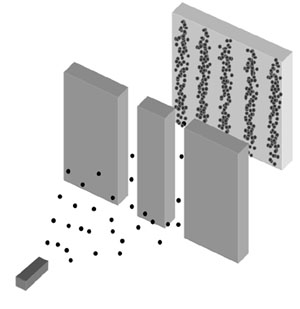
\includegraphics[width=0.5\textwidth]{double-slit-electrons1}
    \caption{visualizzazione dell'esperimento delle due fenditure}
\end{figure}
  
\subsection{Dalla Località alla non Località}
Centrale nella scienza moderna è la nozione che gli oggetti sono affetti direttamente unicamente da forze o oggetti vicini, questa assunzione, 
che nella fisica classica prende il nome di principio di località, non è sempre valida nella fisica quantistica. È possibile infatti
mettere due particelle in una relazione chiamata \emph{entanglement} (le due particelle si diranno entangled) tale per cui: qualsiasi
operazione compiuta su di una avrà un immediato effetto su l'altra anche se queste si trovano ad anni luce di distanza.    

\subsection{Dalle leggi Deterministiche a quelle Non Deterministiche}
Verso quale specifico stato collasserà una sovrapposizione di stati quando misurata? Mentre in altre aree della fisica le leggi sono deterministiche 
i.e. vi è un unico ouput se ripetiamo lo stesso esperimento più volte sotto le stesse condizioni, tuttavia le leggi della meccanica quantistica
ci dicono che possiamo solamente conoscere la probabilità con cui un output, e non un altro, si verificherà. \par

Parafrasando Einstein stesso, queste azioni "spettrali" che emergono nel reame della meccanica quantistica, per quanto radicali ed estranee
alla nostra esperienza quotidiana, sono poi le stesse che, riflettendo la natura esponenziale del mondo sub atomico, conferiscono all'informazione
quantistica il suo vero potenziale. 




\section{Circuiti Booleani}
Ad oggi, il modello a circuiti è l'astrazione per il processo di calcolo più utilizzata nel mondo dell'industria per la progettazione ed il
design delle componenti hardware di un computer.\\
L'unità fondamentale in un circuito Booleano è la porta logica, la quale altro non è che un componente fisico che implementa un operatore della logica di Boole. 
Avremo quindi porte per gli operatori unari come $NOT(\neg)$, per i connettivi binari $AND(\land)$, $OR(\lor)$, $XOR(\xor)$ ecc. . Ogni porta viene rappresentata graficamente 
utilizzando una notazione standard, per esempio: 
\vspace{10pt}
\begin{figure}[h]
    \centering
        \resizebox{.3\textwidth}{!} {%
                    
        \begin{tikzpicture}
            \node (x) at (0, 1) {$x$};
            \node (y) at (0, 0) {$y$};
            
            \node[and gate US, draw, rotate=0, logic gate inputs=nn] at ($(y) + (1.5, 0.5)$) (xandy) {};
            
            

            \draw (x) --  (xandy.input 1);
            \draw (y) -- (xandy.input 2);                
            \draw (xandy.output) -- node[above]{$x *  y$} ($(xandy) + (1.5, 0)$);
            \vspace{-20pt}
        \end{tikzpicture}
        }
        \caption{AND Gate}
    
\end{figure}
\begin{figure}[h]
    \centering
        \resizebox{.3\textwidth}{!}{%
          \begin{tikzpicture}
            \node (x) at (0, 1) {$x$};
            
            \node[not gate US, draw] at ($(x) + (0.8, 0)$) (notx) {};
            
            \draw (x) -- (notx.input);
            \draw (notx.output) -- node[above]{$1-x$} ($(notx) + (1.5, 0)$);
          \end{tikzpicture}
        }
        \caption{AND Gate}
\end{figure}

\noindent sono i simboli che identificano, rispettivamente, la porta AND e la porta NOT.\\
Si noti come la porta AND accetta due proposizioni in input mentre NOT solo una e come l'output rispecchi la funzione calcolata dalla porta, infatti:  \\

\vspace{\abovedisplayskip}
\begin{minipage}{.5\linewidth}
\begin{displaymath}
    \begin{array}{|c|c|}\hline
        (x_1, x_2) & \land{(x_1, x_2)} \\\hline 
        (0, 0)   &  0  \\ 
        (0, 1)   &  0  \\
        (1, 0)   &  0  \\
        (1, 1)   &  1  \\\hline
    \end{array}
    \end{displaymath}
    \captionof{figure}{Tabella di verità per AND}
\end{minipage}
\begin{minipage}{.5\linewidth}
\begin{displaymath}
    \begin{array}{|c|c|}\hline
        x & \neg{(x)} \\\hline 
        0   &  1  \\ 
        1   &  0  \\\hline
    \end{array}
\end{displaymath}
\captionof{figure}{Tabella di verità per OR}
\end{minipage}

\vspace{\belowdisplayskip}
Mettendo in sequenza o in parallelo più porte logiche è possibile esprimere qualsiasi funzione Booleana e, più in generale, qualsiasi funzione calcolabile è rappresentabile mediante
la composizione di una o più porte logiche. Il modello a circuiti è quindi un modello Turing completo.\\
\section{Porte Universali}



 



\begin{thebibliography}{20}
    \addcontentsline{toc}{chapter}{Bibliografia}
    \bibitem{ref1} Higham, N. (1998). \emph{Handbook of writing for the mathematical sciences.} Philadelphia: SIAM, Soc. for Industrial and Applied Mathematics.
    \bibitem{ref2} Encyclopediaofmath.org. (2017). \emph{Boolean function - Encyclopedia of Mathematics.} [online] 
    \bibitem{ref3} Crama, Y. and Hammer, P. (2011). \emph{Boolean Functions Theory, Algorithms and Applications}. 1st ed. Cambridge University Press, p.4.
    \bibitem{ref4} Dobbertin, Hans. \emph{Construction of bent functions and balanced Boolean functions with high nonlinearity.} International Workshop on Fast Software Encryption. Springer, Berlin, Heidelberg, 1994.
    \bibitem{ref5} Logachev, O. A. \emph{On Perfectly Balanced Boolean Functions.} IACR Cryptology ePrint Archive 2007 (2007): 22.
    \bibitem{ref6} Feynmann, R.P. \emph{Simulating physics with computers.} International Journal of Theoretical Physics, 21(6/7):467-488 1982.
    \bibitem{ref7} Benioff, P. \emph{Quantum mechanical models of Turing machines that dissipate no energy.} Physical Reviews Letterers, 48(23):1581-1585, 1982.
\end{thebibliography}
\end{document}


